%!TEX root = ../ausarbeitung.tex
\section{Klassifizierung mit Spatial Pyramid Matching}

\subsection{Grundidee Spatial Pyramid Matching}

Spatial Pyramid Matching ist eine Weiterentwicklung des Bag-of-visual-Words-Ansatzes von Lazebnik et al. \cite{lsp06}. Er wurde 2006 eingeführt und ursprünglich zur Klassifizierung von Szenerien benutzt, um zu erkennen, ob ein Bild beispielsweise eine Stadt, einen Wald oder einen Strand zeigt. Beim Spatial Pyramid Matching werden nicht einfach alle Features ungeordnet betrachtet. Stattdessen wird das Bild in immer feinere Teilbilder unterteilt, deren Features jeweils in einem Spatial Bin gesammelt werden. Der $L_0$-Bin wird in jeder Dimension halbiert und bildet somit vier $L_1$-Bins. Diese wiederum werden wieder geviertelt, was insgesamt 16 $L_2$-Bins bedeutet.

Die Features aus jedem der insgesamt 21 Bins werden anschließend über die Lösung eines Optimierungsproblems den Features eines Codebooks $B$ zugeordnet. Bei dem Codebook handelt es sich um eine Menge von Features, die den Featureraum über der Datenmenge gut widerspiegelt. Dazu werden üblicherweise Features über zufälligen Bildern oder Bildausschnitten der Datenbank berechnet und anschließend mithilfe von Clustering Repräsentanten bestimmt. Bei einigen Verfahren wird das Codebook auch online weiter optimiert, worauf wir jedoch verzichten. Wir haben in unseren Evaluierungen Codebooks mit 256, 512, 1024 und 2048 Features getestet. Je größer das Codebook ist, desto besser können auch komplizierte Datenbanken mit vielen und vielfältigen Klassen abgebildet werden. Auf der anderen Seite steigt die Komplexität der Berechnungen mit größerem Codebook deutlich an.

\begin{figure}
	\centering
	\fbox{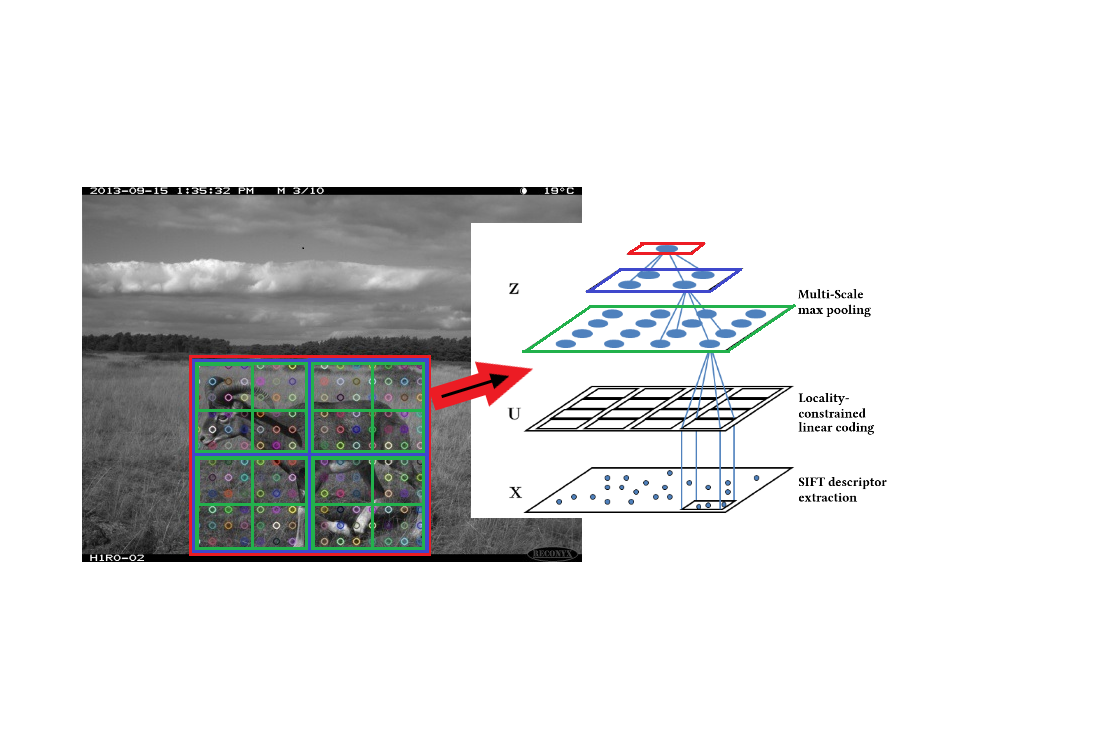
\includegraphics[scale=1]{img/sift_spm.png}}
	\caption{Architektur des Algorithmus mit Veranschaulichung der Spatial Pyramid auf SIFT-Features und Pooling. Im Anschluss werden der $L_0$- (rot), die vier $L_1$- (blau) und 16 $L_2$-Codes (grün) konkateniert - angelehnt an \cite{yygh09}.}
	\label{img:architecture}
\end{figure}

Nachdem für jeden Spatial Bin alle Features mit dem Codebook kodiert wurden, werden diese pro Bin gepoolt, um einen einzige Zuordnung für diesen zu bilden. Die Länge entspricht dabei der Anzahl der Features im Codebook. Abschließend werden die Kodierungen aller Bins konkateniert. Für ein Codebook mit 1024 Features ergibt sich so beispielsweise ein SPM-Code der Länge $21 \cdot 1024 = 21504$. Diese SPM-Codes können dann mit Klassifizierern wie beispielsweise Support Vector Machines (SVMs) eingesetzt werden. Durch die Länge der Codes könnte man erwarten, dass die Laufzeit der Klassifizierung sehr hoch ist. Wie wir im nächsten Abschnitt sehen werden, sind diese gut linear separierbar, weshalb eine SVM mit effizientem linearen Kernel verwendet werden kann. Ein Überblick über das Verfahren befindet sich in Abbildung \ref{img:architecture}.

Unser Algorithmus orientiert sich insgesamt lose an dem Verfahren von \cite{ywkjwh13}. Dort wurden zunächst SIFT- und cLBP-Features dicht auf Bildern berechnet. Mit dem Feature Sign Solver haben sie dann ein dünnbesetztes Kodierungsproblem gelöst \cite{lbrn07}. Die Codes wurden mit Max-Pooling gepoolt, mit der euklidischen Norm normalisiert und anschließend wurden die Bins konkateniert. Die unabhängig voneinander kodierten SIFT und cLBP-Features wurden abschließend mithilfe von AdaBoost und einer linearen SVM klassifiziert.

\subsection{Locality-constrained Linear Coding}

\subsubsection{Grundidee}

Wir verwenden zur Kodierung unserer Features das \emph{Locality-constrained Linear Coding} (LLC) \cite{wyylhg10}. Bei diesem werden jedem Feature $f$ der Spatial Bins mehrere Features des Codebooks zugeordnet, die insgesamt keinen zu großen euklidischen Abstand von $f$ haben dürfen. Bei der ursprünglichen Variante des Spatial Pyramid Matchings wurde lediglich Vektorquantisierung benutzt \cite{lsp06}. Das heißt, dass jedes $f$ dem nächsten Nachbarn im Codebook zugewiesen wird. Unglücklicherweise kommt es dabei zu schlechten Zuordnungen, wenn es beispielsweise keine Feature im Codebook gibt, das zu $f$ ähnlich ist (1) oder wenn zwei recht ähnliche Features $f$ und $g$ unterschiedlichen Features in $B$ zugeordnet werden (2). Fehler dieser Art nennt man \emph{Quantisierungsfehler}.

Eine deutliche Verbesserung stellte das Verfahren von \cite{yygh09}. Beim \emph{SPM based on sparce coding} (ScSPM) wird jedes Feature $f$ anteilig gleich mehreren Features in $B$ zugeordnet. Über einen Regularisierungsterm wird dabei sichergestellt, dass die Kodierungen insgesamt dünnbesetzt sind. Dieser Algorithmus bietet eine deutliche Verbesserung bei Fehlertyp (1), denn möglicherweise lässt sich $f$ durch Kombination mehrerer Features in $B$ besser darstellen. Da lediglich die Dünnbesetztheit (\emph{Sparsity}) der Kodierungen gefordert ist, können weiterhin zwei ähnliche Features durch vollkommen unterschiedliche Kombinationen von Features aus $B$ repräsentiert werden.

Wang et al. haben festgestellt, dass für eine optimale Zuordnung zum Codebook Sparsity allein nicht ausreicht \cite{wyylhg10}. Deshalb stellen sie in ihrem Optimierungsproblem über einen Regularisierungsterm zusätzlich sicher, dass die Zuordnung lokal stattfindet. Die Lokalität stellt gleichzeitig auch die Sparsity sicher, während das Gegenteil nicht immer der Fall ist. Ein Vergleich dieser Strategien befindet sich in Abbildung \ref{img:quant_comp}.

\begin{figure}
	\centering
	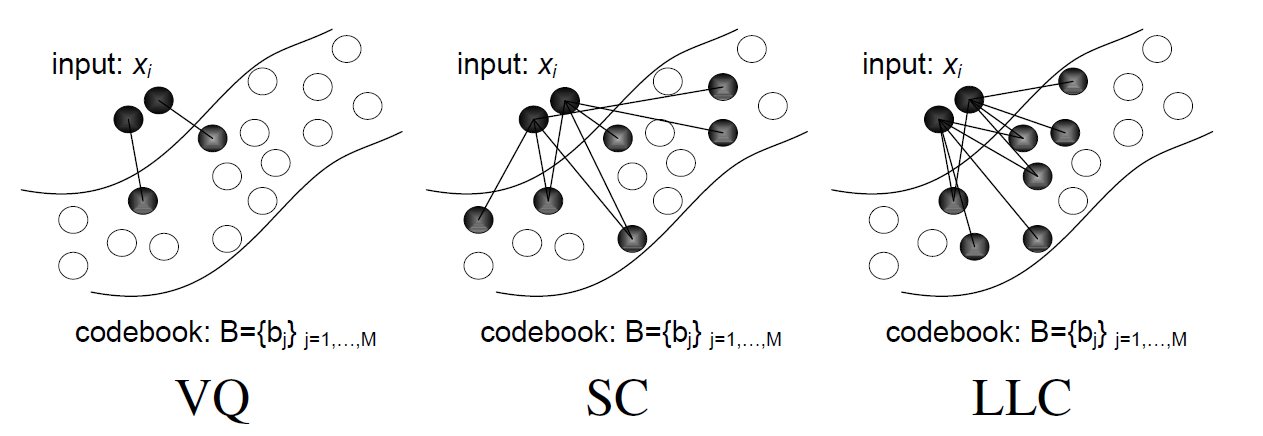
\includegraphics[scale=0.5]{img/quant_comp.png}
	\caption{Vergleich der drei Kodierungsstrategien Vector Quantization, Sparse Coding und Locality-constrained linear Coding \cite{wyylhg10}.}
	\label{img:quant_comp}
\end{figure}

\subsubsection{Optimierungsproblem und analytische Lösung}
\label{sec:llc}

Die Beschreibung von LLC folgt der Veröffentlichung von \cite{wyylhg10}. Es seien eine Menge von D-dimensionalen Features $X = [x_1, \dots, x_N] \in \RR^{(D \times N)}$ und ein Codebook $B = [b_1, \dots, b_M] \in \RR^{(D \times M)}$ mit $M$ Einträgen gegeben. Bei $X$ handelt es sich um Features aus einem Bild und bei $B$ um eine Menge von Deskriptoren, die den Merkmalsraum über allen Bildern gut widerspiegelt.
 
Gesucht ist eine lokale Zuordnung $C = [c_1, \dots, c_N] \in \RR^{(M \times N)}$ von Features aus $X$ auf Visual Words aus $B$. Hierfür verwenden wir das folgende Optimierungsproblem:

\begin{equation}
\min_C \sum_{i=1}^{N} ||x_i - B\cdot c_i||^2 + \alpha\cdot ||d_i \odot c_i||^2, \text{ s.t. } 1^Tc_i = 1 \: \forall \: i
\end{equation}

Betrachten wir den Regularisierungsterm $\alpha\cdot ||d_i \odot c_i||^2$ genauer. $\odot$ ist die elementweise Multiplikation zweier Vektoren. $d_i = \exp \left( \frac{ \mathop{dist}(x_i, B)}{\sigma} \right) \in \RR^{M}$ hingegen ist ein Vektor, der die Distanz des Features $x_i$ zu allen Visual Words aus $B$ angibt. Dabei ist $\mathop{dist}(x_i, B) = [l_2(x_i, b_1), \dots, l_2(x_i), b_m]^T \in \RR^M$ der Vektor der euklidischen Distanzen von $x_i$ zu jedem Visual Word aus $B$. In der Praxis wird $d_i$ zusätzlich normalisiert, indem das Maximum aller $l_2(x_i, b_j)$ bestimmt wird. Dieses wird von jeder Zeile von $\mathop{dist}(x_i, B)$ abgezogen, wodurch sich Werte im Intervall $(-\infty, 0]$ ergeben. Die Anwendung der Exponentialfunktion sorgt dann für normalisierte Distanzwerte in $(0, 1]$. $\alpha$ und $\sigma$ sind Hyperparameter, die bestimmen wie lokal die Zuordnungen sein müssen. \\
Es ist zu beachten, dass die Kodierungen $c_i$ nicht zwangsläufig im Sinne der $l_0$-Norm dünnbesetzt sind. Vielmehr ergeben sich nicht viele relevante Werte, sodass alle zu kleinen Koeffizienten mithilfe eines Thresholds auf 0 gesetzt werden können, um echte Sparsity sicherzustellen. 

Anders als Sparse Coding besitzt LLC eine analytische Lösung und muss nicht mit dem Feature Sign Solver gelöst werden. Als erstes wird die Kovarianzmatrix eines Features $x_i$ über dem Codebook $B$ berechnet, indem wir $x_i$ zeilenweise von $B$ abziehen und die resultierende Matrix mit dem Transponierten seiner selbst multiplizieren:

\begin{equation}
	C_i = (B - 1\cdot x_i^T)\cdot (B - 1\cdot x_i^T)^T
\end{equation}

Die Kovarianzmatrix $C_i$ benutzen wir, um ein lineares Gleichungssystem über dieser Matrix und dem Regularisierungsterm nach $\tilde{c}_i$ zu lösen und anschließend zu normalisieren:

\begin{align}
	(C_i + \lambda\mathop{diag}(d_i)) \cdot \tilde{c}_i &= (1, \dots, 1)^T \\
	c_i &= \tilde{c}_i / 1^T\tilde{c}_i
\end{align}

\cite{wyylhg10} geben die analytische Lösung von LLC als Vorteil gegenüber Verfahren an, die den Feature Sign Algorithmus benutzen, da dieser im besten Fall ein Laufzeit in $\oh(M \cdot K)$ hat, wobei $K$ die Anzahl der Elemente ungleich Null ist. Da $C_i$ nicht dünnbesetzt ist, hat die Lösung des linearen Gleichungssystems im Allgemeinen eine Komplexität von $\oh(M^3)$. Möglicherweise lässt sich das Gleichungssystem mit einem speziellen Solver schneller lösen, da die Kovarianzmatrix symmetrisch und positiv semidefinit ist. In der Praxis hat sich dieser Schritt aber als Flaschenhals des Verfahrens herausgestellt, wie wir in Abschnitt \ref{sec:eval} feststellen werden.

\subsubsection{Pooling und Normalisierung}

Das Resultat von LLC auf eine Menge Featurs $X \in \RR^{(D \times N)}$ ist eine Menge von Kodierungen $C \in \RR^{N \times M}$. $C$ wird auf einen einzelnen trainierten Deskriptor abgebildet, indem wir sie spaltenweise poolen:

\begin{itemize}
	\item sum pooling: $c_{out} = \sum_{i=1}^{N} c_{in, i}$
	\item max pooling: $c_{out} = \max{c_{in, 1}, \dots, c_{in, N}}$
\end{itemize} 

Das Pooling stellt dabei Möglichkeit dar, die Informationen aller Kodierungen aus $C$ in einem Deskriptor zu bündeln und die aussagekräftigsten Informationen dabei zu erhalten. Aufgrund der Assoziativität der Pooling-Operationen ist es nicht nötig alle 21 Bins einzeln zu kodieren. Das erspart einen Menge Aufwand, da jedes Feature aus einem $L_2$-Bin auch in einem $L_1$- und dem $L_0$-Bin auftaucht. Stattdessen reicht es alle $L_2$-Bins einzeln zu kodieren, zu poolen und danach sukzessive das Pooling auf die vier jeweils zusammengehörigen Bins anzuwenden. Dieses \emph{Multi-scale Pooling} wurde auch in Abbildung \ref{img:architecture} veranschaulicht. \\
Zum Abschluss des LLC-Verfahrens werden alle 21 Deskriptoren der einzelnen Bins zu einem einzigen langen LLC-Code konkateniert. Um die Vergleichbarkeit zwischen diesen zu gewährleisten, normalisieren wir sie mit einer der folgenden Methoden:

\begin{itemize}
	\item sum normalization: $c_{out} = c_{in}\: / \: \sum_j c_{in}(j)$
	\item $l^2$ normalization: $c_{out} = c_{in}\: / \: ||c_{in}||_2$
\end{itemize}

\subsubsection{Klassifizierung mit Support Vector Machines}

Die LLC-Codes lassen sich mit einer Support Vector Machine (SVM) mit linearem Kernel klassifizieren. Diese separiert die Klassen mit einer linearen Hyperebene. Ohne auf die Details einzugehen verwenden wir als Loss-Funktion den differenzierbaren \emph{Squared Hinge Loss} und im Falle von mehr als zwei Klassen werden mit der \emph{One-against-all}-Strategie L verschiedene Klassifikatoren trainiert.

Der von uns verwendete lineare Kernel der SVM hat den Vorteil, dass wir den Klassifikator in $\oh(N)$ Zeit trainieren können, während das Testen einen Codes sogar in $\oh(1)$ Zeit möglich ist \cite{yygh09}. Die Laufzeit wird lediglich von der Dimensionalität der Daten, also der Größe des Codebooks bestimmt, nicht aber von der Gesamtanzahl der Features. Demgegenüber benötigen nichtlineare Mercel-Kernels wie beispielsweise der \emph{Chi-square Kernel} oder der im vorigen Kapitel verwendete RBF-Kernel Laufzeiten von $\oh(N^2)$ bis $\oh(N^3)$ fürs Training beziehungsweise $\oh(N)$ fürs Testen. Diese Erkenntnis deckt sich auch mit unseren Evaluierungen, in der das Training der SVM für die Laufzeit des Verfahrens nicht relevant ist. Diese wird stattdessen von der Laufzeit des LLC dominiert.

\subsection{Implementierung}

Die Implementierung des Verfahrens erfolgte in der Programmiersprache Python, wobei verschiedene Bibliotheken zum Einsatz gekommen sind. Zu diesem Zeitpunkt seien uns die Pfade der Bilder und die Regions of Interest der zu klassifizierenden Tiere als Bounding Boxes gegeben. Um die Laufzeit des Verfahrens zu verringern, werden alle Teilbilder auf eine maximale Länge oder Breite von 300 Pixeln verkleinert und in Graustufenbilder umgerechnet. Das Seitenverhältnis bleibt konstant.

\subsubsection{Berechnung der Features}

Wir verwenden zur Klassifizierung der Bilder zwei verschiedene Arten von Features. Das \emph{Scale-invariant-Feature-Transform}-Feature (SIFT) ist ein Strukturfeature, bei dem über eine \emph{Scale-space}-Pyramide von \emph{Difference-of-Gaussian}-Bildern Histogramme von Gradienten berechnet werden \cite{lowe99}. Wir benutzen die Implementierung von OpenCV, die sich in dem Modul \texttt{opencv-contrib} der patentierten Verfahren befindet und gegebenenfalls nicht von sich aus mit OpenCV installiert wird \cite{ocv}. SIFT findet vielfältig Verwendung und zeichnet sich durch hohe Aussagekraft sowie die Invarianz gegenüber Skalierungen und geringen Perspektiv- und Belichtungswechseln aus.

Das zweite Feature ist das Texturfeature \emph{Local Binary Binary} (LBP) \cite{oph94}. Wir verwenden die uniforme Variante mit Radius zwei und 16 benachbarten Punkten von \enquote{Scikit-image} \cite{skimg}. Hierbei wird ein Graustufenpixel mit 16 symmetrisch verteilten Pixel im Abstand von zwei Pixeln verglichen. Falls der Nachbar größer ist als der zentrale Pixel, merken wir uns für diese Stelle eine 0, ist er kleiner, eine 1. Das ergibt bei 16 Nachbarn eine Kodierung von zwei Bytes. In der uniformen Variante prüfen wir zusätzlich, ob der Deskriptor uniform ist, also ob es höchstens zwei Transformationen der Form $0 \rightarrow 1$ oder $1 \rightarrow 0$ gibt. Bei der anschließenden Berechnung des Histogramms über einem Block von Pixeln erstellen wir für jedes uniforme Muster einen Bin im Histogramm und einen einzelnen Bin für alle nicht-uniformen Muster. Die Verwendung der uniformen Variante sorgt dafür, dass die Histogramme lediglich die Länge 18 statt 512 haben und sorgen zusätzlich für Graustufen- und Rotationsinvarianz. 

Die Klasse \texttt{FeatureExtraction} ermöglicht das Berechnen von Featuremengen und Features in Spatial Pyramids für übergebene Featureextraktoren wie beispielsweise dem für SIFT oder LBP. Die Features werden in einem dichten Gitter der Schrittweite 16 über Blöcken von 16 mal 16 Pixeln berechnet. Für die Klassifizierung wäre eine geringere Schrittweite (beispielsweise vier Pixel) vermutlich besser, da bei nicht überlappenden Blöcken wichtige Kanten und Eckpunkte verloren gehen können. Dieses Verfahren wurde auch von \cite{ywkjwh13} verwendet. Wir verzichten bewusst darauf, um die Anzahl der Features und damit die Komplexität der Berechnungen zu verringern.

\subsubsection{LLC Encoding}

Den Kern unseres Verfahrens bildet die Klasse \texttt{LlcSpatialPyramidEncoder}, der über die \texttt{encode}-Methode Features mit LLC kodieren kann. Zuerst wird mithilfe von Scikit-learns \texttt{MiniBatchKMeans} ein Codebook über einer Menge von Features trainiert, die auf der Datenbank der Bilder zufällig bestimmt wurden \cite{sklearn}. Anschließend wurde der Algorithmus aus Abschnitt \ref{sec:llc} mit \enquote{Numpy} umgesetzt. Leider hat sich die Laufzeit der Kodierung als problematisch herausgestellt (s. \ref{sec:eval}), weshalb der ursprünglich sequentielle Algorithmus in klassischem Python mehrmals optimiert wurde. Die Hilfsfunktionen der Klasse wurden in das Modul \texttt{llc\_optimization} ausgelagert und mit \enquote{Numba} annotiert \cite{numba}. Numba bietet die Möglichkeit Pythonfunktionen, die lediglich die Standardbibliothek und Numpy verwenden, mit sogenannten \emph{Decorators} zu markieren. Bei der Ausführung des Programms werden diese Funktionen mit Hilfe des LLVM-Compilers in Echtzeit kompiliert, was in einer deutlich schnelleren Laufzeit im Vergleich zu interpretiertem Code resultiert. 

\subsubsection{Scikit-learn SPM-Transformer und LinearSVC}

Alle obigen Funktionen wurden in der Klasse \texttt{SpmTransformer} zusammengefasst. Diese implementiert als Unterklasse von Scikit-learns \texttt{BaseEstimator} die Methoden \texttt{fit} und \texttt{transform}, wodurch sich das LLC-Verfahren problemlos in Scikit-learns \emph{Pipelines} integrieren lässt \cite{sklearn}. Das ermöglicht einem spielend leicht die Kombination mit Klassifizierern, Ensemblemethoden und Modelselektionsverfahren der Bibliothek. \\
Abschließend wurde in dem Modul \texttt{spatial\_pyramid\_matching} das komplette Verfahren von der Segmentierung, über Locality-constrained linear Coding bis zur Klassifizierung mit Scikit-learns \texttt{LinearSVC} auf zwei verschiedenen Datenbanken umgesetzt.